\chapter{Modelagem geral do sistema} \label{chap:modelagem} % 3

% Tendo esclarecido sobre as \hyperref[chap:marco]{questões gerais da área de estudo} e de \hyperref[chap:instituicao]{como se estrutura a instituição} agora nos aprofundaremos na conceitualização do funcionamento geral do sistema e a forma como se dará a execução da \hyperref[sec:Metodologia]{metodologia proposta} apresentando o funcionamento geral de como o sistema será estruturado e de como foi desenvolvido.

Ao longo deste capítulo serão abordados os \hyperref[sec:estagios]{estágios de execução} sobre como se dão as etapas de criações de grade horária no geral, a \hyperref[sec:interacao]{interação} com os \textit{stakeholders}, o \hyperref[sec:funcionamento]{funcionamento} do sistema, o \hyperref[sec:ModelagemBD]{modelo de banco de dados} e a \hyperref[sec:REST]{API REST} que será utilizada para a comunicação entre o \textit{frontend} e o \textit{backend} do sistema.

\section{Estágios de execução} \label{sec:estagios} % 3.1

Em seu trabalho de aplicação prática, \citeonline{Miranda2012} estruturaram estágios que compõem o processo necessário para que enfim se alcance a definição de tabelas horárias finais.

\begin{CenteredFigure} \caption{Estágios para a obtenção de grade horária} \label{fig:geral}
  \includegraphics[width=\textwidth]{files/img/2.02!4-modelagem/Estágios Grade Final}
  \legend{Fonte: \citeonline{Miranda2012} - adaptado}
\end{CenteredFigure}

Na \autoref{fig:geral}, estão dispostos 4 estágios principais. O primeiro dispõe da aquisição de informações, sendo elas a disponibilidade do professor, os recursos da infraestrutura, as grades dos cursos, as estimativas de demanda e as políticas internas. No segundo estágio são definidas grades horárias preliminares com atribuição preliminar das salas. No terceiro, os alunos se inscrevem e a demanda é ajustada, por fim, no quarto estágio, ocorre a alocação final das salas. Com sua conclusão, são definidos as grades horárias finais junto com as respectivas salas.

A sequência geral condiz com o processo de criação das grades horárias, porém é necessário adaptar a metodologia para o contexto da UENF, e também ao escopo do trabalho. Os recursos de infraestrutura serão coletados dos histórico de alocação das turmas, a estimativa de demandas será obtida através da média histórica de alunos inscritos nas turmas e as políticas internas serão compreendidas através da revisão documental e entrevistas com os \textit{stakeholders}. O segundo tem caráter iterativo entre as coordenações e a diretoria do CCT. Os outros estágios não se distanciarão de forma significativa do que foi proposto.

\section{Interação} \label{sec:interacao} % 3.2

Para se alcançar uma alta satisfação por parte dos \textit{stakeholders}, vê-se necessária a constante interação com os mesmos. Para isto, será seguida a estrutura utilizada por \citeonline{Andre2018}.

\begin{CenteredFigure} \caption{Etapas do Design de Interação} \label{fig:IxD}
  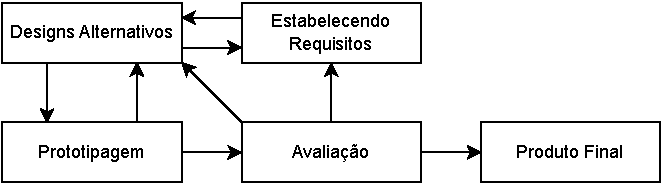
\includegraphics{files/img/2.02!4-modelagem/Arquitetura-IxD}
  \legend{Fonte: \citeonline{Andre2018} - adaptado}
\end{CenteredFigure}

Seguindo o conceito do Design de Interação, a \autoref{fig:IxD} ilustra o ciclo de ações a serem tomadas durante o desenvolvimento do sistema, caso este venha a ser necessário. Nesse modelo de pesquisa, os \textit{stakeholders} serão consultados continuamente enquanto lhes for apresentados protótipos do sistema, para que assim informem quanto às suas percepções. Esta dinâmica tem como finalidade encontrar um design tal que seja adequado aos desejos e necessidades de seus usuários. Pois, considerando que para que o sistema seja efetivo, é necessário que ele seja aceito e utilizado pelos usuários finais.

\section{Funcionamento} \label{sec:funcionamento} % 3.3

O sistema proposto funcionará de forma a auxiliar a coordenação do curso de Ciência da Computação da UENF na criação de grades horárias para os semestres letivos. Para isso, o sistema deverá ser capaz de gerenciar as informações referentes às disciplinas, professores, salas e horários disponíveis.

Para tanto, mesmo que disponha de informações pré-cadastradas, o sistema deverá permitir a inserção de novas informações, como disciplinas, professores e salas, pois, apesar de não ser o foco principal do sistema, é recorrente que haja alterações nessas informações ao longo do tempo, e caso o sistema não as comporte, não poderá cumprir seu propósito.

Como forma de agregar as informações cadastradas, o usuário será capaz de criar turmas para as disciplinas, informando o professor responsável, a sala e o horário em que a turma ocorrerá. Além disso, o sistema deverá permitir a visualização das turmas já cadastradas, bem como a edição e exclusão das mesmas, caso necessário. Ao criar uma turma, o sistema viabiliza a definição de qual ano e semestre a turma pertence.

As turmas contarão também com a informação de demanda estimada, que será utilizada como comparativo para a alocação das salas, de forma a evitar que uma sala seja alocada para uma turma cuja demanda seja maior do que a capacidade da sala. Outra informação contida nas turmas será um código descritor da turma em questão. Esse código será utilizado para auxiliar na compreensão das turmas, visto que ao longo do processo de criação das grades horárias é recorrente a criação de turmas criadas com um propósito específico, como por exemplo contemplar apenas repetentes ou alunos de um determinado conjunto de cursos.

Como ponto chave do funcionamento do sistema, o mesmo deverá ser capaz de ilustrar conflitos que vierem a surgir durante a alocação dos recursos. Esses conflitos podem ser de diversas naturezas, como por exemplo, a alocação de uma turma em um horário em que o professor responsável não está disponível, ou a alocação de duas turmas em uma mesma sala e horário. A identificação desses conflitos é essencial para que a coordenação possa corrigí-los de forma prática e direta, assim evitando que ocorram problemas durante a execução das turmas no semestre letivo.

Por fim, o sistema viabiliza também um método de rápida criação de turmas para todas as disciplinas esperadas para determinado semestre letivo para o curso de Ciência da Computação. Esse método consiste em analisar as disciplinas esperadas para os estudantes de computação em determinado semestre letivo, e, através do cálculo das maiores recorrências de professor, sala e horário atribuídos às turmas dessa mesma disciplina em semestres anteriores, criar uma turma com essas informações. Esse método visa agilizar o processo de criação das turmas, visto que a coordenação não precisará criar cada turma manualmente, mas sim apenas revisar as informações geradas pelo sistema.

Dispondo de todas essas funcionalidades, o sistema deverá ser capaz de gerar uma grade horária final, que será utilizada como base para a criação da grade horária oficial do curso de Ciência da Computação da UENF.

\section{Modelo de banco de dados} \label{sec:ModelagemBD} % 3.4

Considerando as informações necessárias para o presente trabalho, e também o preparo de campo para potenciais aplicações futuras, foi elaborado um diagrama conceitual parcial do banco de dados (\autoref{fig:DiagramConceitual}). Seu intuito foi trazer uma visualização mais clara das relações entre as entidades presentes no processo de criação de uma grade horária, e assim auxiliar na definição das tabelas que serão criadas no banco de dados \hyperref[ssssec:MySQL]{posteriormente}.

\begin{MyCenteredFigure} \caption{Diagrama Conceitual do banco de dados} \label{fig:DiagramConceitual}
  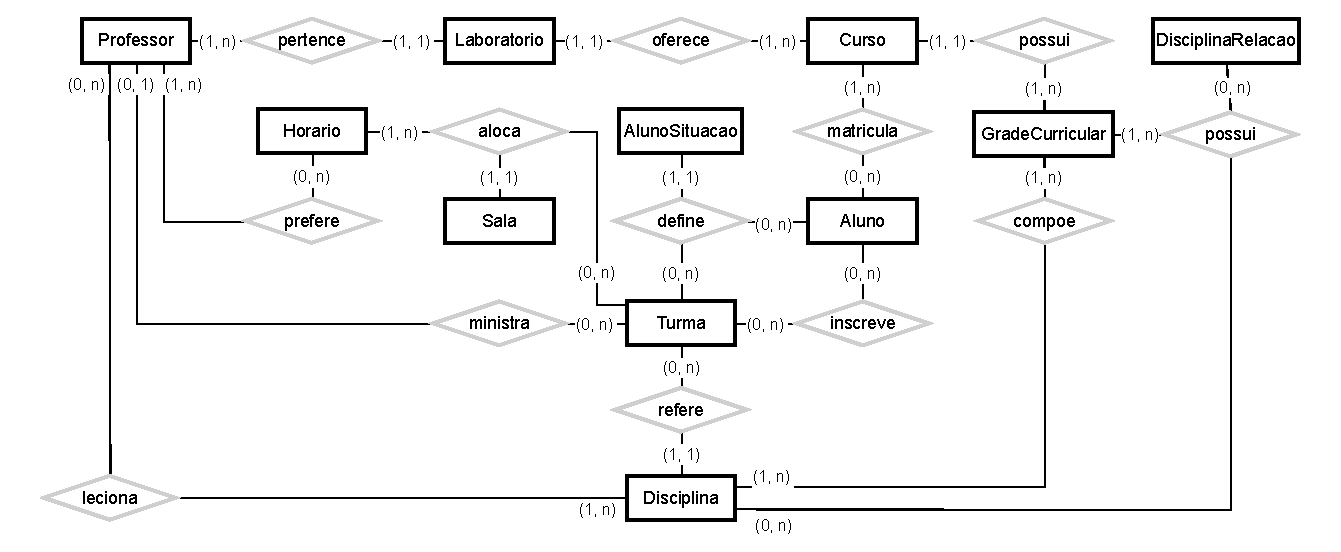
\includegraphics[width=\textwidth]{files/img/2.02!4-modelagem/Diagrama Conceitual}
\end{MyCenteredFigure}

O diagrama conceitual foi desenvolvido utilizando a ferramenta \LinkToURL{\LinkDrawio}{draw.io} e ilustra as relações entre diversas entidades presentes na realidade da UENF. O emaranhamento presente no diagrama ilustra a complexidade envolvida na criação de uma grade horária, onde diversas entidades se relacionam entre si.

Como principais apontamentos, podemos citar a parte principal do modelo que é a entidade \textbf{turma}. Ela, como já descrito, envolve a correlação entre alunos de diferentes cursos, professores, disciplinas, salas e horários. Além disso, também é possível notar a presença de entidades que não são diretamente relacionadas à alocação de turmas, mas que podem se mostrar úteis no futuro, como a relação entre professores e laboratórios; e a de disciplinas e ementas.

Embora o diagrama apresente uma visão mais completa das interconexões possíveis, é importante ressaltar que o presente trabalho foca primordialmente na alocação das turmas para o curso de Ciência da Computação, e que a implementação do banco de dados será feita de forma a atender a essas necessidades, fazendo então uso de apenas uma parte do diagrama conceitual apresentado pela \autoref{fig:DiagramConceitual}.
Sendo posteriormente ilustrados na \autoref{ssec:MVP2} pela \autoref{fig:TabelasIniciais}, na \autoref{ssec:MVP3} pela \autoref{fig:MVP3_BancoDeDados} e na \autoref{ssec:Funcionalidades preparadas} pela \autoref{fig:DER final}.
% Sendo posteriormente ilustrados na \hyperref[ssec:MVP2]{subseção ``Versão 2.0''} pela \autoref{fig:TabelasIniciais}, na \hyperref[ssec:MVP3]{subseção ``Versão 3.0''} pela \autoref{fig:MVP3_BancoDeDados} e na \hyperref[ssec:Funcionalidades preparadas]{subseção ``Funcionalidades preparadas''} pela \autoref{fig:DER final}.

% DEIXAR MAIS DESCRITO EM QUE SEÇÃO ESSAS FIGURAS ESTÃO.

% \subsection{Diagrama de Entidade e Relacionamento} % 3.4.1

% Neste modelo, mais enxuto, temos apenas as entidades principais, onde temos uma turma de determinada disciplina, ministrada por um professor e que ocorre em uma sala em um determinado horário.

% Neste diagrama vemos as entidades principais, que são \textbf{Turmas}, \textbf{Disciplinas}, \textbf{Professores}, \textbf{Horários} e \textbf{Salas}. As propriedades escolhidas para cada entidade são compostas por uma mistura de critérios. Por exemplo, o nome do professor, o código da disciplina, e a junção de código e bloco auxiliam primordialmente na identificação real dos professores, disciplinas e salas. Já as informações ``período'', ``apelido'' e ``comment''...

% E também é notável a presença da entidade \textbf{Alunos}, que se apresenta desacoplado das demais entidades. O motivo para isso é que, embora os alunos façam parte do processo de alocação de turmas, ao longo do desenvolvimento, o desenvolvimento de funcionalidades envolvendo os alunos...

\section{API REST} \label{sec:REST} % 3.5

Para exemplificar o funcionamento geral da permanência dos dados, consideremos o uso de uma \textbf{API REST} (Application Programming Interface, em português: Interface de Programação de Aplicações) (Representational State Transfer, em português:  Transferência de Estado Representacional) utilizando de 4 ``camadas'': o \textbf{\textit{frontend}}, os \textbf{\textit{endpoints}}, as \textbf{funções} de execução e o \textbf{banco de dados}.

% Essa parte sobre Dev e Prod tá muito deslocada
% Ele se encontra em duas formas: a primeira é o chamado ``em produção'', que é o sistema que o usuário final acessa, e a segunda é o chamado ``em desenvolvimento'', que é o sistema que o desenvolvedor acessa para realizar as modificações necessárias. Ambas precisam

O \textbf{\textit{frontend}} é a interface do sistema, onde o usuário interage com o sistema. Essa interface precisa se comunicar com o \textit{backend} para realizar as quatro operações básicas no banco de dados (criação, leitura, atualização e deleção) por sobre as entidades existentes (turmas, professores, disciplinas, salas, etc.). Elas assim o fazem ao enviar requisições HTTP (\textit{GET}, \textit{POST}, \textit{PUT} e \textit{DELETE}), contendo pacotes de informações em formato JSON para os \textbf{\textit{endpoints}}.

Os \textbf{\textit{endpoints}} são as rotas que o \textit{backend} disponibiliza para a recepção das requisições HTTP. Eles são responsáveis por encaminhar as requisições recebidas. Seu funcionamento consiste em rotear as requisições recebidas junto com sua carga útil. Para tanto, as rotas criadas refletem diretamente a qual entidade do banco de dados a requisição se refere, sendo então assim sabido qual \textbf{função} deve ser executada.

As \textbf{funções} são as responsáveis por executar as operações no banco de dados. Elas processam o pacote de informações recebido, e então realizam a operação desejada no \textbf{banco de dados}.

O \textbf{banco de dados} recebe a requisição, processa a operação, e então retorna o status da operação. Esse retorno é então repassado camada por camada, até chegar ao \textit{frontend}, onde o usuário final pode visualizar o resultado da operação.

\textbf{Resumidamente}: O \textbf{\textit{frontend}} envia uma requisição HTTP com uma carga de informações a um \textbf{\textit{endpoint}}, que encaminha a requisição a uma \textbf{função} específica que executa uma operação no \textbf{banco de dados}, assim retornando o status da operação ao \textit{frontend}.

\section{Diferença dos trabalhos anteriores} \label{sec:diferenca} % 3.6

Os trabalhos mais próximos ao presente, quanto a instituição são os trabalhos feitos por \citeonline{SanyaSantos2013} e \citeonline{RicardoSilveira2014}, porém, o presente trabalho se distingue em algumas questões.

Talvez uma das mais marcantes distinções é a visualização presente nos dois trabalhos anteriores onde são considerados um limite de cinco disciplinas por horário, pois ambos consideram em seus trabalhos que o curso de computação está dividido entre as cinco turmas de cada grupo de períodos, sejam as do semestre ímpar (1, 3, 5, 7 e 9) ou as do semestre par (2, 4, 6, 8 e 10). No entanto, o presente trabalho avalia que, é mais condizente com a realidade da instituição se for considerado que os alunos tendem a não seguir completamente essa subdivisão, tendendo a ficar com disciplinas de semestres diferentes geralmente aquém do esperado, mas também podendo estar além do que se espera.

Outra característica marcante é a dependência de salas disponíveis que comportem o número de alunos esperados para a turma, o que não é considerado pelos autores, visto que esta característica não é vista como pertencente ao escopo da Coordenação do Curso de Ciência da Computação. Já neste trabalho, considera-se que esta informação é essencial para que haja a confirmação da validade da alocação da turma. Além disso, como existem diversos outros cursos que utilizam as salas do CCT, é importante que a coordenação tenha conhecimento sobre a disponibilidade das salas para que possa alocar as turmas de forma eficiente, sendo então necessário o preenchimento de informações sobre as disciplinas necessárias para os outros cursos.

Existem também alguns critérios usados por \citeonline{SanyaSantos2013} e \citeonline{RicardoSilveira2014} que não são considerados no presente trabalho, como a preferência de professores associados e professores contratados, e o desejo por se evitar alocar disciplinas que possuam aulas em horários próximos ou que sobreponham o horário de almoço.
